\subsection{Softmax regression development results}
Across the 870 outer-fold predictions, softmax accuracy is 90.80\% and macro-F1 is 0.9081. Mean outer accuracy is 90.80\% with sample fold SD 2.60 percentage points; outer-fold accuracies range from 88.51\% to 94.83\%. Mean outer-training accuracy is 95.72\%, indicating a training-validation gap. Aggregate log loss is 0.2452; unlike accuracy, it also reflects the probabilities assigned to the true classes.

\begin{center}
\begin{tabular}{lrrrr}
\toprule
Sport & Precision & Recall & F1 & Support \\
\midrule
Baseball & 0.8889 & 0.9103 & 0.8995 & 290 \\
Basketball & 0.9241 & 0.9241 & 0.9241 & 290 \\
Soccer & 0.9117 & 0.8897 & 0.9005 & 290 \\
\bottomrule
\end{tabular}
\end{center}

There are 80 errors. The largest directed confusions are Soccer predicted as Baseball (19 rows); Baseball predicted as Soccer (17 rows). 8 wrong predictions assign at least 0.9 probability to the predicted class, showing that confidence alone does not guarantee correctness. Fixed keyword flags omit unmatched language and a linear classifier cannot represent every feature interaction; these are structural limitations rather than established causes of individual errors.

These are development cross-validation results for softmax, not untouched-test results or a final family selection. Preliminary exploration informed keyword definitions before an untouched local test group could be verified, so earlier feature design may make estimates optimistic. Final model selection and the single-number hidden-test performance estimate await the tuned decision-tree and random-forest results.

% Optional figure for the combined report; preserve the one-page Results limit.
% 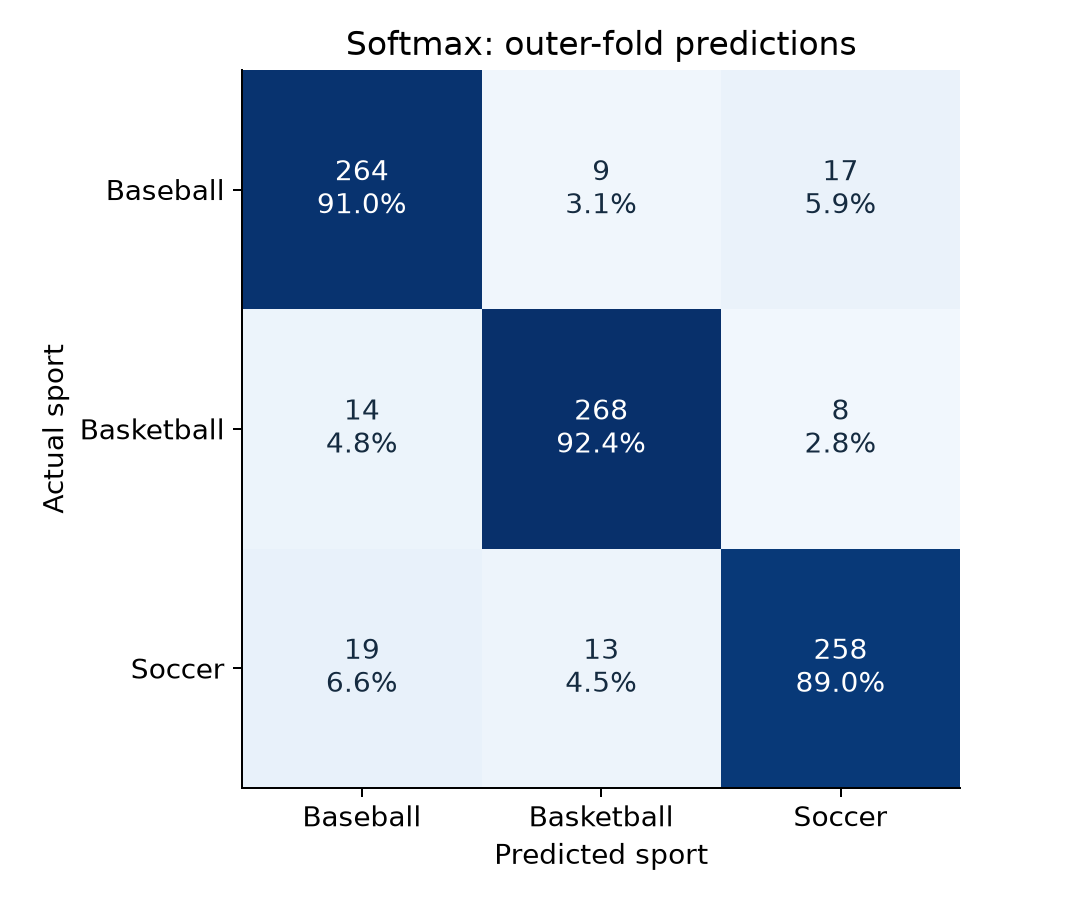
\includegraphics[width=.55\linewidth]{results/softmax/figures/confusion_matrix.png}
